\documentclass[margin=5pt]{standalone}
% \usepackage[a4paper]{geometry}
\usepackage[utf8]{inputenc}
\usepackage{xifthen}
\usepackage{tikz}
% \usetikzlibrary{patterns}
\usetikzlibrary{math,calc}

\title{16 possible outcomes}
\author{Stuart Presnell}
\date{November 4th 2020}


% Modelling the 2^4 possible outcomes in the 4 remaining undeclared swing states

\begin{document}
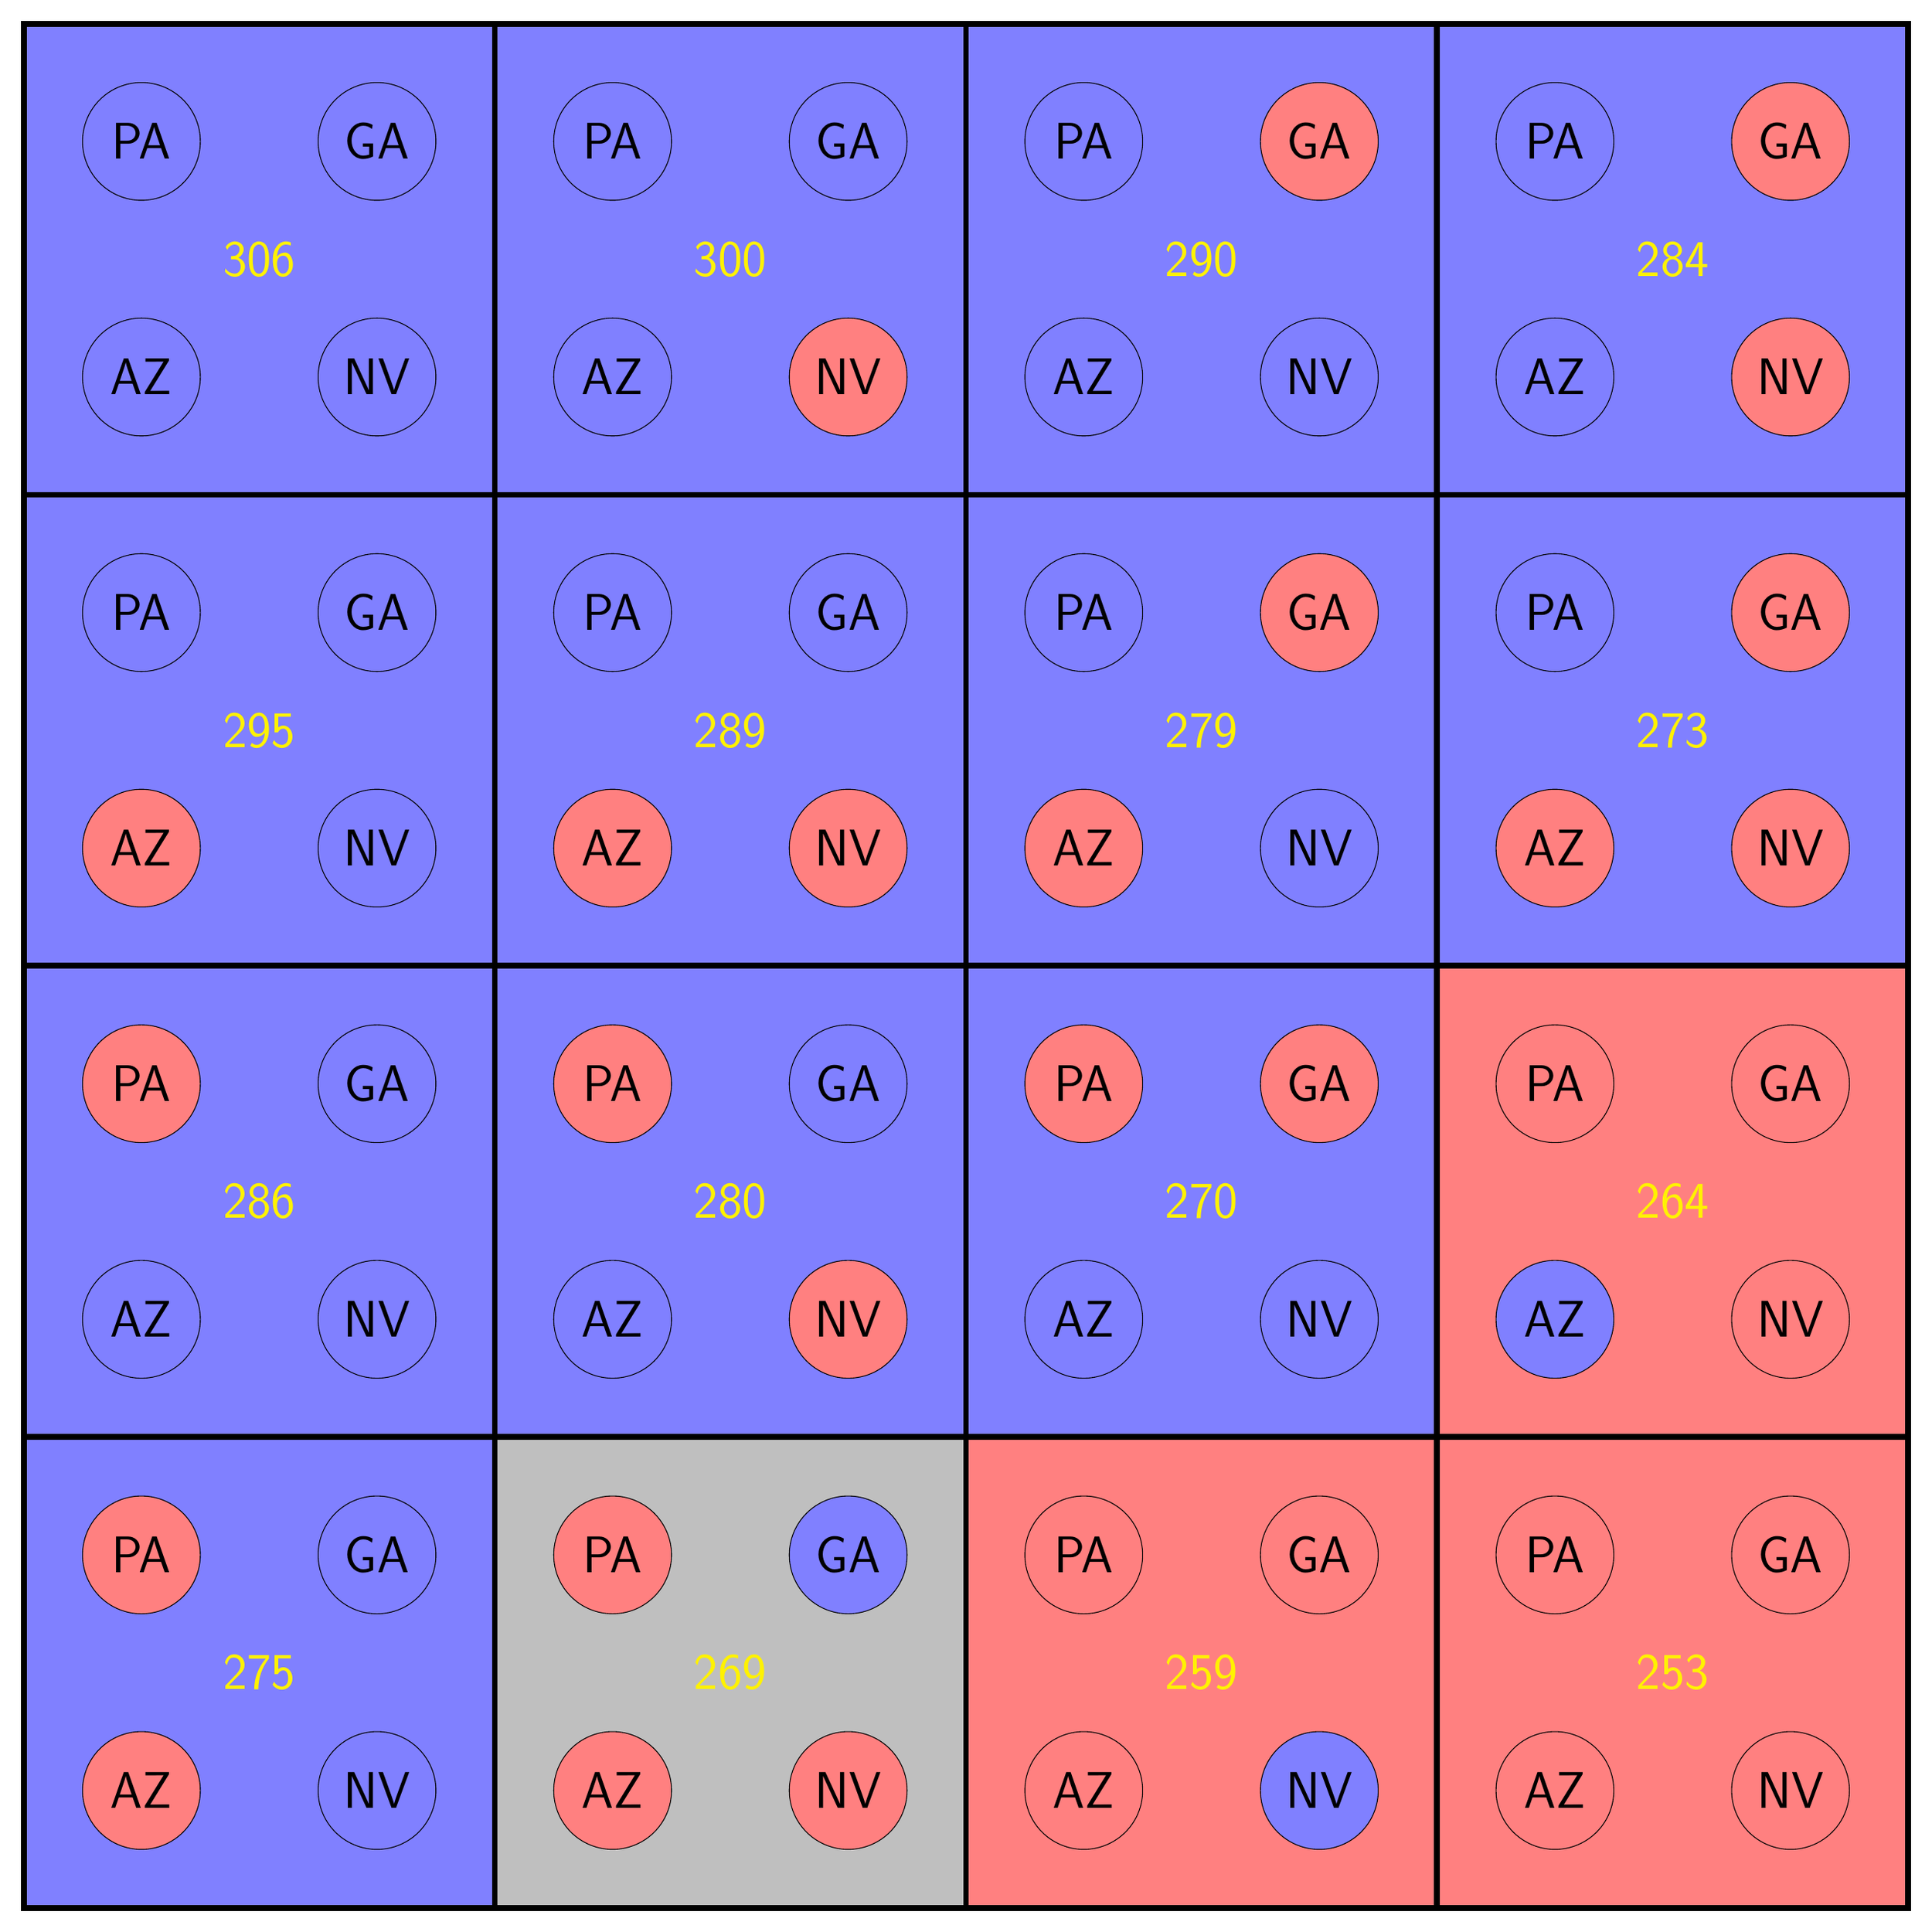
\begin{tikzpicture}\sffamily
\def\xmin{0};
\def\xmax{32};
\def\ymin{0};
\def\ymax{32};


% Grid:
\draw[step=1cm,gray,dotted,thick] (\xmin,\ymin) grid (\xmax,\ymax);

% Style for the labels of the state circles and for the EC total in each box
\tikzstyle{label}=[font=\Huge, text=black]

\tikzstyle{Dwin}=[fill=blue!50]
\tikzstyle{Rwin}=[fill=red!50]
\tikzstyle{tied}=[fill=gray!50]


% The diagram is a grid of 4x4 boxes, each depicting a possbile outcome
% This command draws a single box

\newcommand{\drawbox}[8]{
% #1, #2 = xcoord, ycoord of lower left corner of box
% #3, #4, #5, #6 = Outcome in GA, PA, NV, AZ
% #7 = Number of EC votes for Dem
% #8 = Overall outcome

% Draw an 8x8 box at the given position, coloured for the overall outcome
\draw[line width=1mm, #8] (#1,#2) rectangle ++(8,8);

% Write the Number of EC votes in the centre of the box
\coordinate (score) at ($(#1,#2)+(4,4)$);
\node[label, text=yellow] at (score) {#7};

% Now we draw the 4 circles in the box, each corresponding to a state
% They're placed at +2 or +6 from the lower left corner of the box
% Each state's circle is coloured according to its winner in this scenario
\coordinate (GA) at ($(#1,#2)+(6,6)$);
\draw[#3] (GA) circle (1cm);
\node[label] at (GA) {GA};

\coordinate (PA) at ($(#1,#2)+(2,6)$);
\draw[#4] (PA) circle (1cm);
\node[label] at (PA) {PA};

\coordinate (NV) at ($(#1,#2)+(6,2)$);
\draw[#5] (NV) circle (1cm);
\node[label] at (NV) {NV};

\coordinate (AZ) at ($(#1,#2)+(2,2)$);
\draw[#6] (AZ) circle (1cm);
\node[label] at (AZ) {AZ};
} % End of definition of `drawbox`


% Now draw the 16 boxes
% This enumeration of the possible outcomes and their EC totals was calculated by hand
% Perhaps there's a way to automate this?
\drawbox{0}{0}{Dwin}{Rwin}{Dwin}{Rwin}{275}{Dwin}
\drawbox{0}{8}{Dwin}{Rwin}{Dwin}{Dwin}{286}{Dwin}
\drawbox{0}{16}{Dwin}{Dwin}{Dwin}{Rwin}{295}{Dwin}
\drawbox{0}{24}{Dwin}{Dwin}{Dwin}{Dwin}{306}{Dwin}
\drawbox{8}{0}{Dwin}{Rwin}{Rwin}{Rwin}{269}{tied}
\drawbox{8}{8}{Dwin}{Rwin}{Rwin}{Dwin}{280}{Dwin}
\drawbox{8}{16}{Dwin}{Dwin}{Rwin}{Rwin}{289}{Dwin}
\drawbox{8}{24}{Dwin}{Dwin}{Rwin}{Dwin}{300}{Dwin}
\drawbox{16}{0}{Rwin}{Rwin}{Dwin}{Rwin}{259}{Rwin}
\drawbox{16}{8}{Rwin}{Rwin}{Dwin}{Dwin}{270}{Dwin}
\drawbox{16}{16}{Rwin}{Dwin}{Dwin}{Rwin}{279}{Dwin}
\drawbox{16}{24}{Rwin}{Dwin}{Dwin}{Dwin}{290}{Dwin}
\drawbox{24}{0}{Rwin}{Rwin}{Rwin}{Rwin}{253}{Rwin}
\drawbox{24}{8}{Rwin}{Rwin}{Rwin}{Dwin}{264}{Rwin}
\drawbox{24}{16}{Rwin}{Dwin}{Rwin}{Rwin}{273}{Dwin}
\drawbox{24}{24}{Rwin}{Dwin}{Rwin}{Dwin}{284}{Dwin}


\end{tikzpicture}
\end{document}
